110%% The following is a directive for TeXShop to indicate the main file
%%!TEX root = diss.tex

%%%%%%%%%%%%%%%%%%%%%%%%%%%%%%%%%%%%%%%%%%%%%%%%
\chapter{Experimental and Analysis Techniques}
\label{ch:techniques}
%%%%%%%%%%%%%%%%%%%%%%%%%%%%%%%%%%%%%%%%%%%%%%%%

The measurement of internal conversion coefficients depends on accurate analysis of $\gamma$-ray and electron spectra. For an individual transition between nuclear states, the relative transition probability by different transition modes must be calculated. This depends fundamentally on fitting mathematical functions to the spectroscopic peak structures that we have identified as belonging to specific transitions. This peak fitting is described in detail in Section \ref{sec: Peak Fitting}. The approach to calibrating the efficiencies of the detectors used in collection of the experimental data is then discussed in Section \ref{sec: Calibration of Detection Efficiency}. Calculations of previously unmeasured internal conversion coefficients must be normalized based on existing measurements, as well as the relative efficiency of our detectors. A simulated efficiency curve for the SPICE detector, using the GEANT4 toolkit, is discussed in Section \ref{sec: Simulated SPICE Efficiency}. This normalization, and the techniques used for determining internal conversion coefficients, are discussed in Section \ref{sec: Determining Internal Conversion Coefficients}. The calculation of electric monopole transition strengths, $\rho^2(E0)$, and associated error analysis are discussed in Section \ref{sec:Determining E0 Transition Strengths}.

%%%%%%%%%%%%%%%%%%%%%%%%%%%%%%%%%%%%%%%%%%%%%%%%
\section{Experimental Details}
\label{sec: Experimental Details}
% !!! For now this is mostly a copy of James' writing. This isn't the focus, so we're leaving it as is. It could easily be expanded using Daniel's style later.
%%%%%%%%%%%%%%%%%%%%%%%%%%%%%%%%%%%%%%%%%%%%%%%%

In June of 2016, a beam of 35.6\,MeV alpha particles with a typical intensity of 120\,ppA was delivered by the TRIUMF-ISAC-II superconducting linear accelerator to the TIGRESS spectrometer. The beam was incident on a self-supporting $^{110}$Pd target of 1.6\,mg/cm$^2$ with a 97.61\% isotopic enrichment. The target was positioned 8\,mm upstream of the nominal center of the TIGRESS spectrometer.

Two micron S3 silicon detectors of 140\,$\mu$m and 1000\,$\mu$m thickness were located downstream in a $\Delta E-E$ telescope configuration to detect and identify charged particles. Twelve of the TIGRESS high-purity germanium (HPGe) clover detectors were positioned around the target location to detect $\gamma$ rays. Four clovers were located at 45$^{\circ}$ with respect to the beam axis, and the remaining eight at 90$^{\circ}$ \cite{Hackman14}.

The spectrometer for internal conversion electrons (SPICE) detector was used to detect internal conversion electrons emitted from excited states populated in the reaction. The main detector of SPICE is a 6.1\,mm thick lithium-drifted silicon (Si(Li)) detector shielded by a photon shield from direct sight of the target. A magnetic lens formed of rare-earth permanent magnets collects and directs internal conversion electrons around the photon shield into the Si(Li) detector. The annular detector with inner and outer radii of 1 and 10\,cm is segmented into 120 individual segments arranged with 12 azimuthal sectors and 10 rings.

Figure \ref{figure: TIGRESS and SPICE schematic} provides a schematic diagram of the experimental setup, showing the incident $\alpha$ beam, TIGRESS, SPICE, the $^{110}$Pd target, and the downstream S3 detector.

\begin{figure}[!ht]
  \centering
  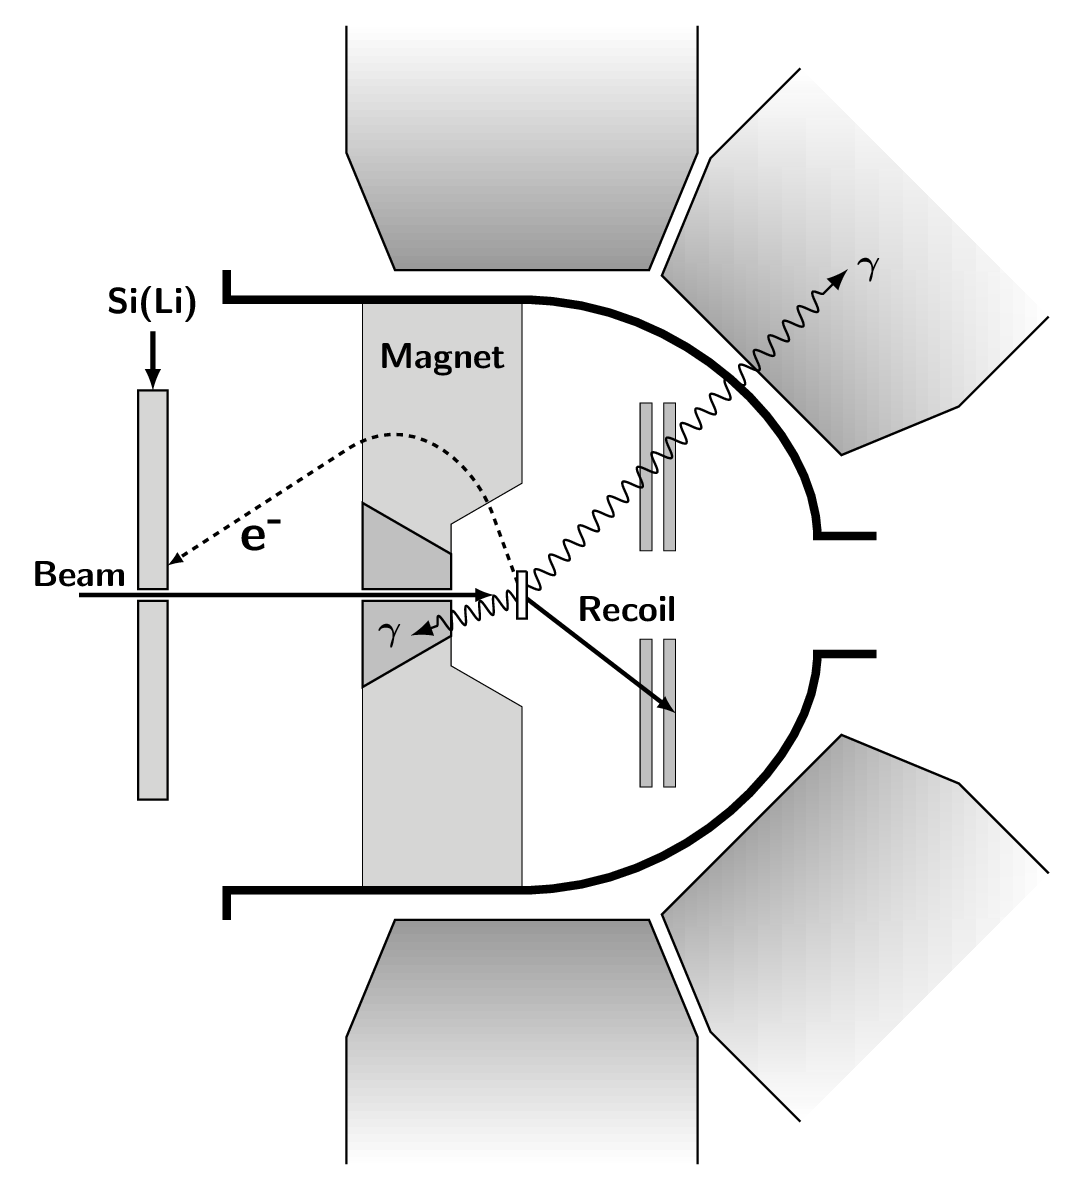
\includegraphics[width=0.8\textwidth]{techniques_spice_schematic.png}
  \caption[Schematic diagram of the experimental apparatus used in the June 2016 $\alpha$ particle scattering experiment at TRIUMF's ISAC-II facility.]{Schematic diagram of TIGRESS and SPICE in ISAC-II. An incoming beam of particles, $\alpha$ in this experiment, is shown colliding with the target, $^{110}\mathrm{Pd}$, at the center of the apparatus. As the excited target nuclei decay down to the ground state, they emit electrons ($e^-$) that follow curved trajectories through the internal magnetic fields of SPICE and are then detected by the upstream Si(Li) detectors. When $\gamma$-ray photons are emitted they are detected by the TIGRESS clovers, trapezoidal in the schematic, while the recoiling nuclei are detected by a downstream S3 silicon detector.}
  \label{figure: TIGRESS and SPICE schematic}
\end{figure}

Due to the above-Coulomb-barrier reaction energy of the collisions, excited nuclear states of several different nuclei were populated. Figure \ref{figure: nuclear chart region} shows the region of the nuclear chart where $^{110}\mathrm{Pd}$ and the other populated nuclei are found. The nuclei populated in this experiment are highlighted in orange.

\begin{figure}[!ht]
  \centering
  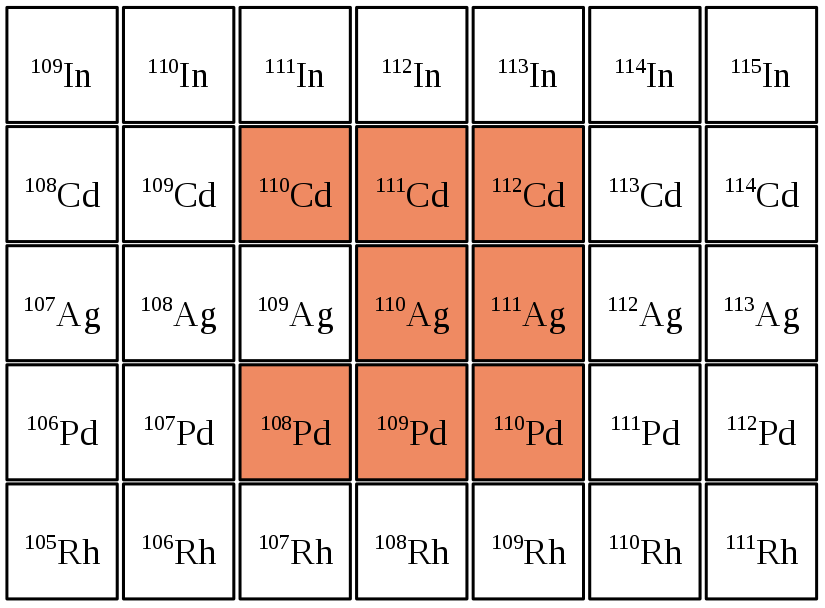
\includegraphics[width=0.7\textwidth]{techniques_chart_region.png}
  \caption[A chart of nuclides in the region of $^{110}\mathrm{Pd}$; highlighting the nuclei observed in the experiment.]{A chart of nuclides in the region of $^{110}\mathrm{Pd}$. The nuclei observed in this experiment are highlighted in orange.}
  \label{figure: nuclear chart region}
\end{figure}

The $\gamma$-ray and $e^-$ spectra for $^{110}$Pd is shown in Figure \ref{figure:spectrum_sample}. For both plots the spectrum presented is of all particles detected in time coincidence with a specific range of $\alpha$ particle energy, as detected in the S3. Three transitions are highlighted in each spectrum. All the denoted $e^-$ peaks are from $K$ shell electrons, except for the discernible $L$ shell peak from the $2^+_1 \rightarrow 0^+_1$ transition. 

\begin{figure}[!ht]
  \centering
  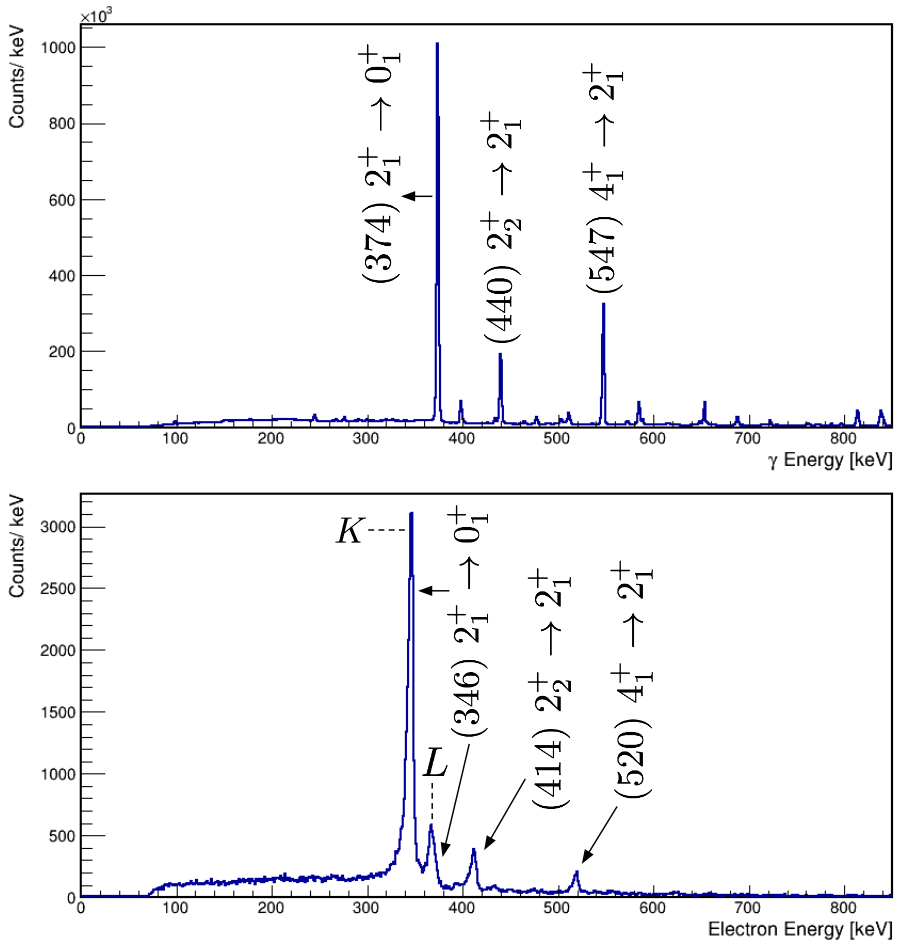
\includegraphics[width=0.9\textwidth]{techniques_alpha_spectra.png}
  \caption[The $\alpha$-particle gated $\gamma$-ray spectrum and the $\alpha$-particle gated $e^-$ spectrum.]{$\gamma$-ray and $e^-$ energy spectra for $^{110}$Pd from TIGRESS and SPICE. These spectra were produced by gating on a specific range of $\alpha$ particle energies, as detected in the S3 detector. Three transitions are highlighted in each spectrum, with the discernible $K$ and $L$ peaks for the $2^+_1 \rightarrow 0^+_1$ transition annotated. The energy listed for that transition, 346 keV, refers specifically to the $K$ peak.}
  \label{figure:spectrum_sample}
\end{figure}

%%%%%%%%%%%%%%%%%%%%%%%%%%%%%%%%%%%%%%%%%%%%%%%%
\section{Peak Fitting}
\label{sec: Peak Fitting}
%%%%%%%%%%%%%%%%%%%%%%%%%%%%%%%%%%%%%%%%%%%%%%%%

In both the $e^-$ and $\gamma$-ray spectra, the peaks have low-energy tails. This is due to incomplete charge collection in the detectors. The low energy tails of the $e^-$ peaks are likely to be due to target straggling and back-scattering. In both the $e^-$ and $\gamma$-ray spectra, the peak shapes may be described by regular Gaussian functions, $g(x)$, where

\begin{gather}
g(x) = e^{-\big(\frac{x-x_0}{\sigma \sqrt{2}}\big)^2}
\label{equation: Gaussian definition}
\end{gather}

summed with a skewed Gaussian, $d(x)$, to account for the low-energy tail from incomplete charge collection effects where

\begin{gather}
d(x) = e^{\big(\frac{x-x_0}{\beta}\big)} \cdot \mathrm{erfc}\Bigg[\frac{x-x_0}{\sigma \sqrt{2}} + \frac{\sigma}{\beta \sqrt{2}}\Bigg]
\label{equation: skewed Gaussian definition}
\end{gather}

where $x_0$ is the peak's centroid value, $\sigma$ is the width of the Gaussian and $\beta$ controls the length of the tail \cite{Radford2016}. The error function, erf($x$), is part of the integration of a normal distribution i.e.

\begin{gather}
\mathrm{erf}(x) = \frac{2}{\sqrt{\pi}}\int^x_0 e^{-t^2}\mathrm{d}t
\label{equation: erf(x) definition}
\end{gather}

and the complimentary error function, erfc, that appears in equation (\ref{equation: skewed Gaussian definition}), is simply $1-\mathrm{erf}(x)$ \cite{AndrewsText}.

Figure \ref{figure: example 2 to 0 fit} shows an example fit from the $e^-$ spectrum of the dataset, where there are overlapping peaks within a small energy region. The need to fit multiple peaks arises frequently, particularly in the $e^-$ data where the separation energy between the $K$ and $L$ atomic electron shells in $^{110}\mathrm{Pd}$ is 20.82 keV, which is determined from the difference between corresponding atomic-shell binding energies \cite{KIBEDI2008202}. In Figure \ref{figure: example 2 to 0 fit} the ratio of intensities between the $K$ and $L$ peaks is not constrained. By leaving this ratio of intensities as a free parameter, the measurement of the $L$ peak can be used in the calculation of a separate internal conversion coefficient which can then be utilized in the normalization procedure to be described in Section \ref{sec: Determining Internal Conversion Coefficients}. Here the dashed blue area in the fit highlights the use of an exclusion area, where there appears to be some structure but it is not definitively peak like, nor does it correspond to any identified nuclear transitions. The region is omitted from the fit in order to improve accuracy of the included measurements.

\begin{figure}[!ht]
  \centering
  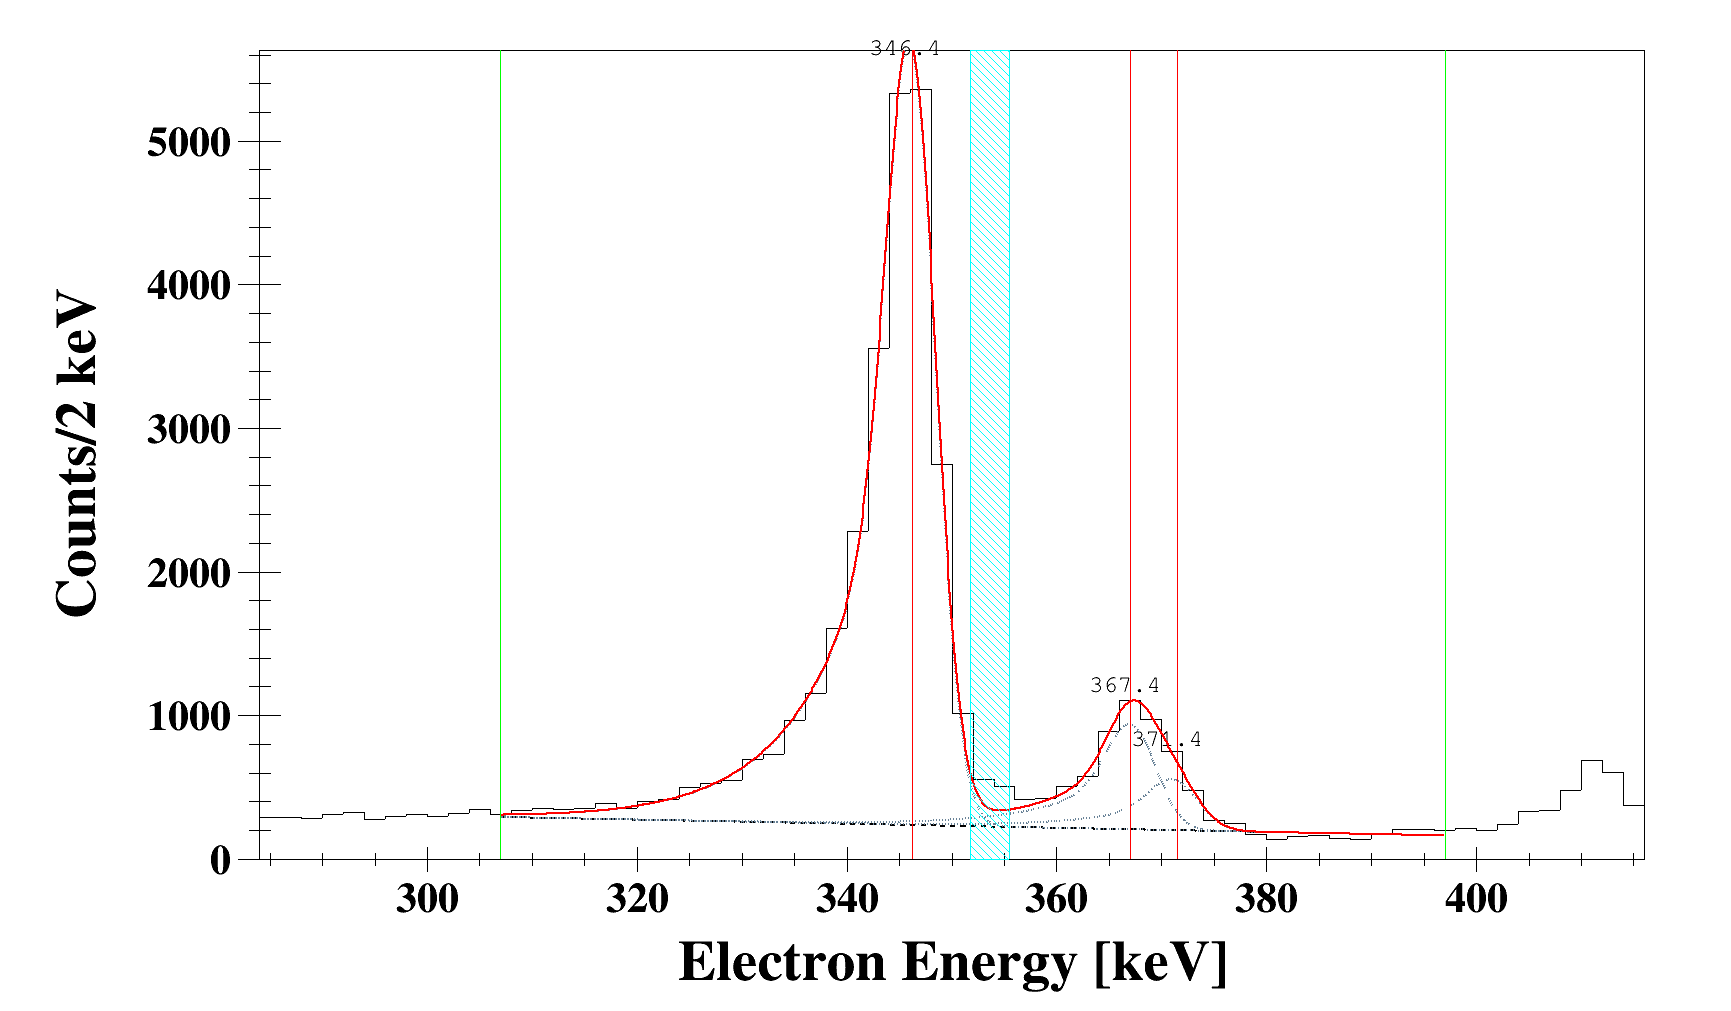
\includegraphics[width=\textwidth]{techniques_fit_example.png}
  \caption[An example of simultaneously fitting three peaks in the $\alpha$-energy gated $e^-$ data. The $K$ to $L$ peak intensity ratios are unconstrained.]{An example of simultaneously fitting three peaks in the $\alpha$-energy gated $e^-$ data. The major peak at 346.4 keV corresponds to $K$ shell electrons from the $2^+_1 \rightarrow 0^+_1$ transition in $^{110}\mathrm{Pd}$. The $L$ peak for this transition lies at 367.4 keV, while the peak at 371.4 keV was identified as belonging to a $(3^+) \rightarrow 2^+$ transition (parentheses denote a tentative multipolarity assignment), also from $^{110}\mathrm{Pd}$, with $\gamma$-ray energy of 398.6 keV. In this fit the energy separations between all peaks are fixed, but the inter-peak height ratios are not. The red vertical lines denote the peak centroids used by the fitting program, the green lines delimit the energy range considered by the fit, and the dashed blue area highlights an area of data that was excluded from the fit.}
  \label{figure: example 2 to 0 fit}
\end{figure}

There are fits for which constraining the $K$ to $L$ peak intensity ratio becomes necessary, an example of this is shown in Figure \ref{figure: example constrained fit}. The close clustering of peak structures from several identified transitions renders the use of an intensity constraint unavoidable. Hence, only a $K$ peak measurement is carried forward to the normalization procedure as an independent measurement. 

\begin{figure}[!ht]
  \centering
  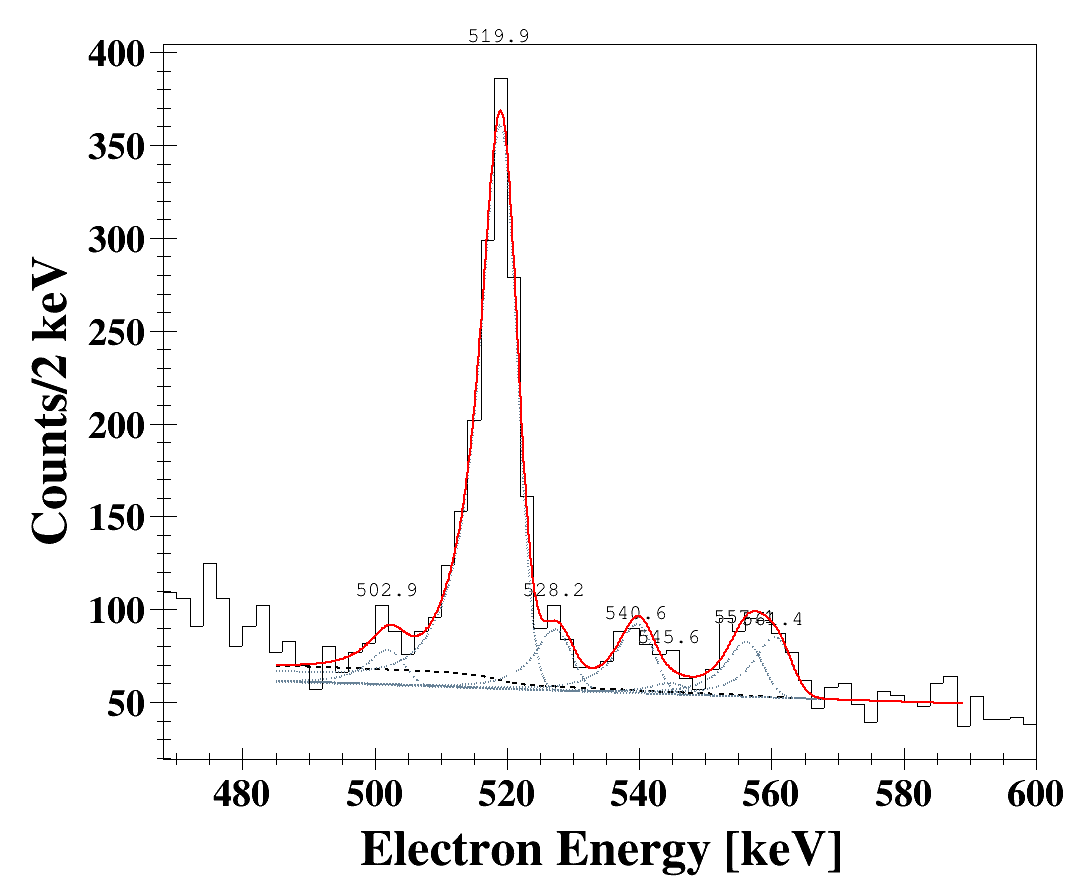
\includegraphics[width=\textwidth]{techniques_fit_constrained.png}
  \caption[An example of simultaneously fitting seven peaks in the $\alpha$-energy gated $e^-$ data. The $K$ to $L$ peak intensity ratios are constrained.]{An example of simultaneously fitting seven peaks in the $\alpha$-energy gated $e^-$ data. Here the peak at 519.9 keV is the $K$ shell peak for the $4^+_1 \rightarrow 2^+_2$ transition in $^{110}\mathrm{Pd}$. The corresponding $L$ peak is at 540.6 keV. There are several other identified transitions with peak structures present and included in the fit. The intensity ratio between the $K$ and $L$ peaks of the transitions of interest is constrained using the theoretical values from BrIcc \cite{KIBEDI2008202}.}
  \label{figure: example constrained fit}
\end{figure}

Figures \ref{figure: example 2 to 0 fit} and \ref{figure: example constrained fit} show data that is obtained by performing an energy gate on the recoiling $\alpha$ particle detected by the downstream S3 detector. Gating on an $\alpha$ particle amounts to selecting out only those $e^-$ that were detected, by SPICE, coincident in time with an $\alpha$ particle in the S3 detector. In this example a further pruning of the spectrum is achieved by gating on a specified range of $\alpha$ particle energies. This technique applies equally to the analysis of $\gamma$-ray spectra, and must be applied equivalently in form when measuring internal conversion coefficients, i.e. a direct comparison of intensities from the two types of radiated particles. 

The $\Delta E - E$ particle identification plot from the S3 detectors is shown in Figure \ref{figure: particle ID with alpha energy}. The experimental setup included multiple S3 detectors arranged in a telescope configuration that allows for the identification of particles based on their differential energy loss. The elastic peak, the highest intensity point at {\raise.17ex\hbox{$\scriptstyle\sim$}} 3600 keV total energy, corresponds predominantly to false coincidence between the elastic $\alpha$ particle beam, and the radiation from inelastic reaction products such as the Cd isotopes. Hence, two protons have been transferred to the $^{110}$Pd target, and some number of neutrons are detected by the S3. Moving along the intensity curve, upward in $\Delta E$ and leftward in $E$, inelastic, Coulomb excitation reactions exciting $^{110}$Pd to successively higher energy states are observed. The decay radiation from these states is observed in coincidence with an S3 detected $\alpha$ recoil. Nearing the end of this curving feature, the highest $\Delta E$ particles detected correspond to inelastic scattering of a high enough energy to dislodge neutrons from the target. These neutrons, and the incident $\alpha$ particle, are detected in coincidence with radiation from the nuclei $^{109}$Pd and $^{108}$Pd. The separate features, in the lower ranges of both $\Delta E$ and $E$, correspond to inelastic reactions wherein a single proton from the incident $\alpha$ particle is captured by a target nucleus, and the recoiling proton, deuteron (one proton, one neutron), or tritium (one proton, two neutrons) is detected in the S3 along with the possible free neutron products. These detections are coincident with the radiation emitted by the Ag isotopes. 

\begin{figure}[!ht]
  \centering
  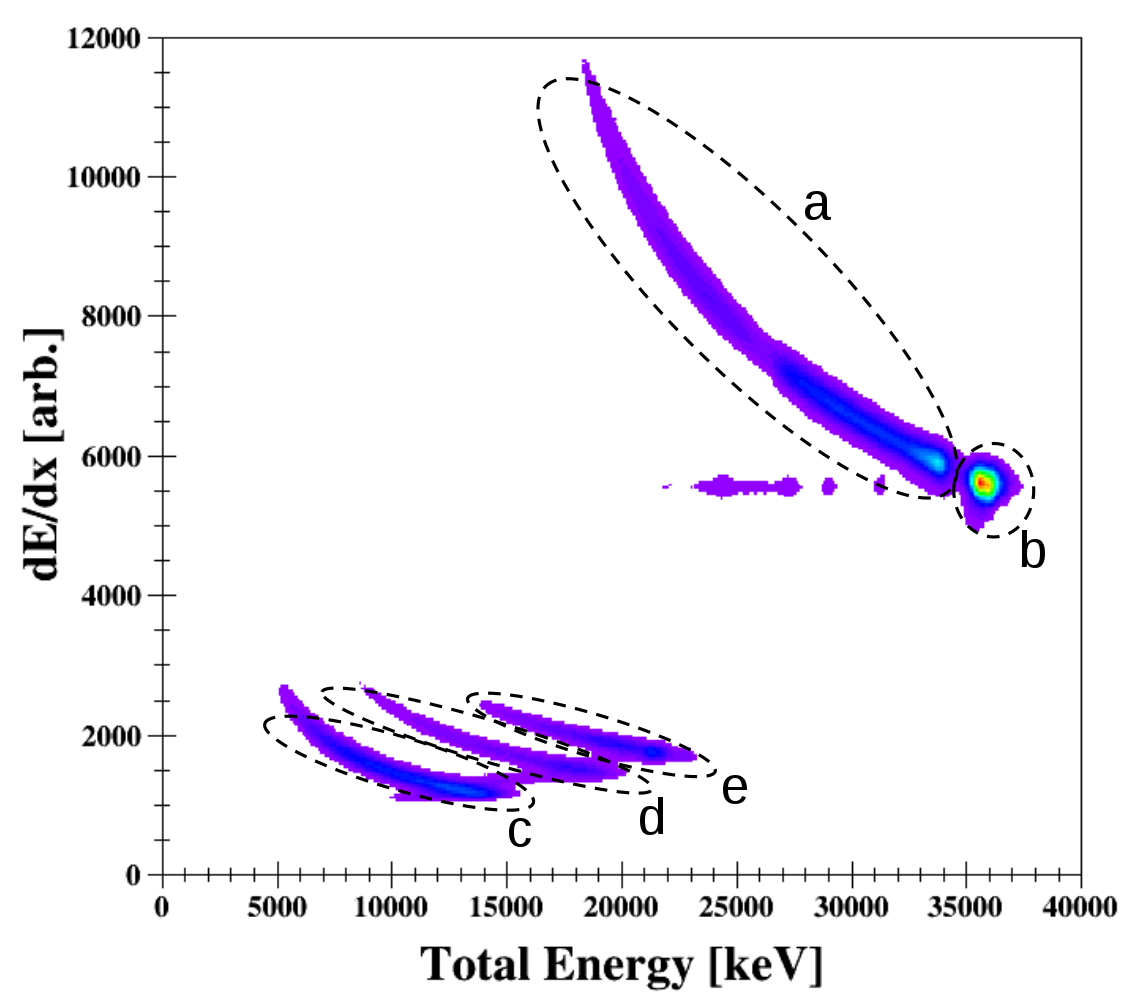
\includegraphics[width=\textwidth, height=0.84\textwidth]{techniques_particle_ID.png}
  \caption[$\Delta E - E$ particle identification plot from the S3 telescope.]{$\Delta E - E$ particle identification plot from the S3. The experimental setup included multiple S3 detectors arranged in a telescope configuration that allows for the identification of particles based on their differential energy loss: a) Inelastic, Coulomb excitation reactions, exciting $^{110}$Pd to successively higher energy states. Nearing the end of this curving feature, the highest $\Delta E$ detections are inelastic scattering $\alpha$ particles coincident with the nuclei $^{109}$Pd and $^{108}$Pd. b) The elastic peak, corresponding predominantly to random coincidence between the elastic $\alpha$ particle beam, and the radiation from inelastic reaction products such as the Cd isotopes. The separate features, c, d, and e, correspond to detected protons, deuterons, and tritons, respectively. These are inelastic reactions wherein a single proton from the incident $\alpha$ particle is captured by a target nucleus. These detections are coincident with the radiation emitted by the Ag isotopes.}
  \label{figure: particle ID with alpha energy}
\end{figure}

Gating on the energy range in detected $\alpha$ particles presented a sufficiently clean, i.e. removing enough of the unwanted transitions and background, $\gamma$-ray and $e^-$ spectra for the internal conversion coefficient analysis. All of the spectra fitting analysis was performed using an analysis package called jRootAnalysisTools, developed at TRIUMF, and built upon the ROOT data analysis framework \cite{Brun1997}.

%%%%%%%%%%%%%%%%%%%%%%%%%%%%%%%%%%%%%%%%%%%%%%%%
\section{Calibration of Detection Efficiency}
\label{sec: Calibration of Detection Efficiency}
%%%%%%%%%%%%%%%%%%%%%%%%%%%%%%%%%%%%%%%%%%%%%%%%

To be assured of accuracy of experimental data, a calibration of the SPICE detector using radioactive source data was necessary. Both before and after the experimental campaign, a radioactive $^{207}\mathrm{Bi}$ source was used in calibration. $^{207}\mathrm{Bi}$ is chosen because it has an intense, easily resolvable, internal conversion electron spectrum. The 120 individual segments of the SPICE Si(Li) detector were reviewed for there accuracy of reproducing the expected $^{207}$Bi electron spectrum. 9 channels were deemed to be ineffective, and were removed from the final data set sorted for analysis.

All of the data for the experimental analysis was sorted using a sorting program called GRSIsort, developed by the Gamma-Ray Spectroscopy at ISAC (GRSI) group \cite{GRSIsort}. 

%%%%%%%%%%%%%%%%%%%%%%%%%%%%%%%%%%%%%%%%%%%%%%%%
\section{Simulated SPICE Efficiency}
\label{sec: Simulated SPICE Efficiency}
%%%%%%%%%%%%%%%%%%%%%%%%%%%%%%%%%%%%%%%%%%%%%%%%

The TIGRESS and SPICE detectors have unique particle detection efficiencies. In order to make absolute measurements of physical events, the efficiency of the detectors must be considered. If the $\gamma$-ray and $e^-$ efficiencies were equivalent, then any error resulting from detection inefficiencies would cancel. It is the relative efficiency between the two detectors that matters. This can be seen explicitly from the way that the internal conversion coefficient is calculated

\begin{gather}
\alpha_K= \frac{A_e}{A_\gamma} \cdot \frac{\epsilon_\gamma}{\epsilon_e}
\label{equation: ICC and Efficiency}
\end{gather}

where $A_e$ and $A_\gamma$ are the measured $e^-$ and $\gamma$-ray counts. The $\gamma$-ray detection efficiency, $\epsilon_\gamma$, of TIGRESS is well characterized, via a previous efficiency calibration with $^{152}\mathrm{Eu}$, $^{133}\mathrm{Ba}$, $^{207}\mathrm{Bi}$, and $^{56}\mathrm{Co}$ sources. The $e^-$ efficiency, $\epsilon_e$, of SPICE must be determined by making measurements of internal conversion coefficients for which the transition multipolarity is known. The relative difference between these measurements and the expected values calculated by BrIcc will provide information on the efficiency of $e^-$ detection in the experiment. Additionally, the approximate shape of the SPICE efficiency curve, as it changes with incident $e^-$ energy, can be determined from simulation in Geant4. The combination of normalization from previously measured values, and an understanding of the shape of efficiency changes with energy, provides a method for calculating previously unmeasured internal conversion coefficients. 

Geant4 is a toolkit for the simulation of the passage of particles through matter \cite{Geant4}. Using a package specific to the SPICE detector, simulations at $e^-$ energies spanning the SPICE detection range were performed \cite{detectorSimulations}. The results for this simulation are shown in Figure \ref{figure: SPICE simulated efficiency}. 

% !!! The inclusion of a Geant4 viewer image with particle tracks could do

\begin{figure}[!ht]
  \centering
  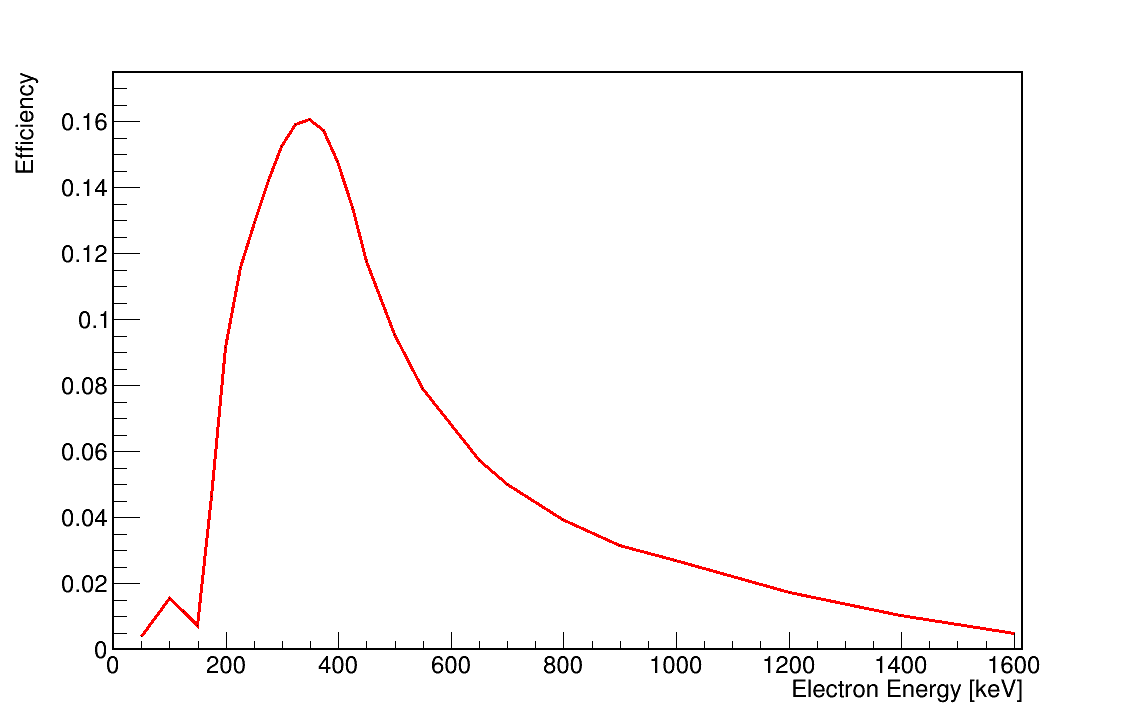
\includegraphics[width=\textwidth]{techniques_spice_simulation.png}
  \caption[A simulation of the SPICE detection efficiency using the Geant4 toolkit.]{A simulation of the SPICE detection efficiency using the Geant4 toolkit \cite{detectorSimulations,Geant4}.}
  \label{figure: SPICE simulated efficiency}
\end{figure}

% !!! The efficiency changes with beam spot characterization is could be added

% Further investigation of the resulting efficiency was undertaken. Two parameter spaces were explored in additional simulations: changing the circular area of the $e^-$ source, and moving the position of that source off of the beam line axis. The position and size of the $e^-$ source is meant to correspond to the cross-section of the incident beam particles, $\alpha$ in this experiment. The assumption of a perfectly tuned beam, i.e. directly along the axis at which the $^{110}\mathrm{Pd}$ target is placed, is investigated here. In Figures [!!!, !!!, !!!, !!!] the dimensions of the $e^-$ source is shown in conjunction with the resultant simulated SPICE efficiency curve. 

% \begin{figure}[!ht]
%   \centering
%   
\includegraphics[width=\textwidth]{placeholder.png}
%   \caption{Messing around with beam spot, several images [!!!]}
%   \label{figure: beam spot and simulated efficiency}
% \end{figure}


%%%%%%%%%%%%%%%%%%%%%%%%%%%%%%%%%%%%%%%%%%%%%%%%
\section{Determining Internal Conversion Coefficients}
\label{sec: Determining Internal Conversion Coefficients}
%%%%%%%%%%%%%%%%%%%%%%%%%%%%%%%%%%%%%%%%%%%%%%%%

For each observed transition, the number of counts in $e^-$ and $\gamma$-ray spectra is measured, and Equation (\ref{equation: ICC and Efficiency}) was used to calculate an absolute internal conversion coefficient.

The $\gamma$-ray detection efficiency, $\epsilon_\gamma$ is taken from the previously calculated efficiency curve for TIGRESS. The $e^-$ detection efficiency of SPICE was determined by using normalization transitions in order to interpolate the detector efficiency for transitions of interest. Figure \ref{figure: SPICE efficiency normalization with ICC measurements} plots the calculated efficiency and $K$ shell $e^-$ energy for the normalization transitions used, along with an exponential scaling of the simulated SPICE efficiency curve described in Section \ref{sec: Simulated SPICE Efficiency}. The scaling amounts to fitting the following function to the measured internal conversion coefficient data:

\begin{gather}
f(x) =  \epsilon_e(x) \cdot p_1 \cdot e^{\frac{-x}{p_0}} \cdot
\label{equation: exponential scaling}
\end{gather}

where $p_1$ and $p_0$ are parameters to be fit, the variable $x$ stands in for $e^-$ energy, and $\epsilon_e(x)$ is the simulated SPICE efficiency curve. The normalization transitions used are listed in Table \ref{table:norm_icc}.

\begin{figure}[!ht]
  \centering 
  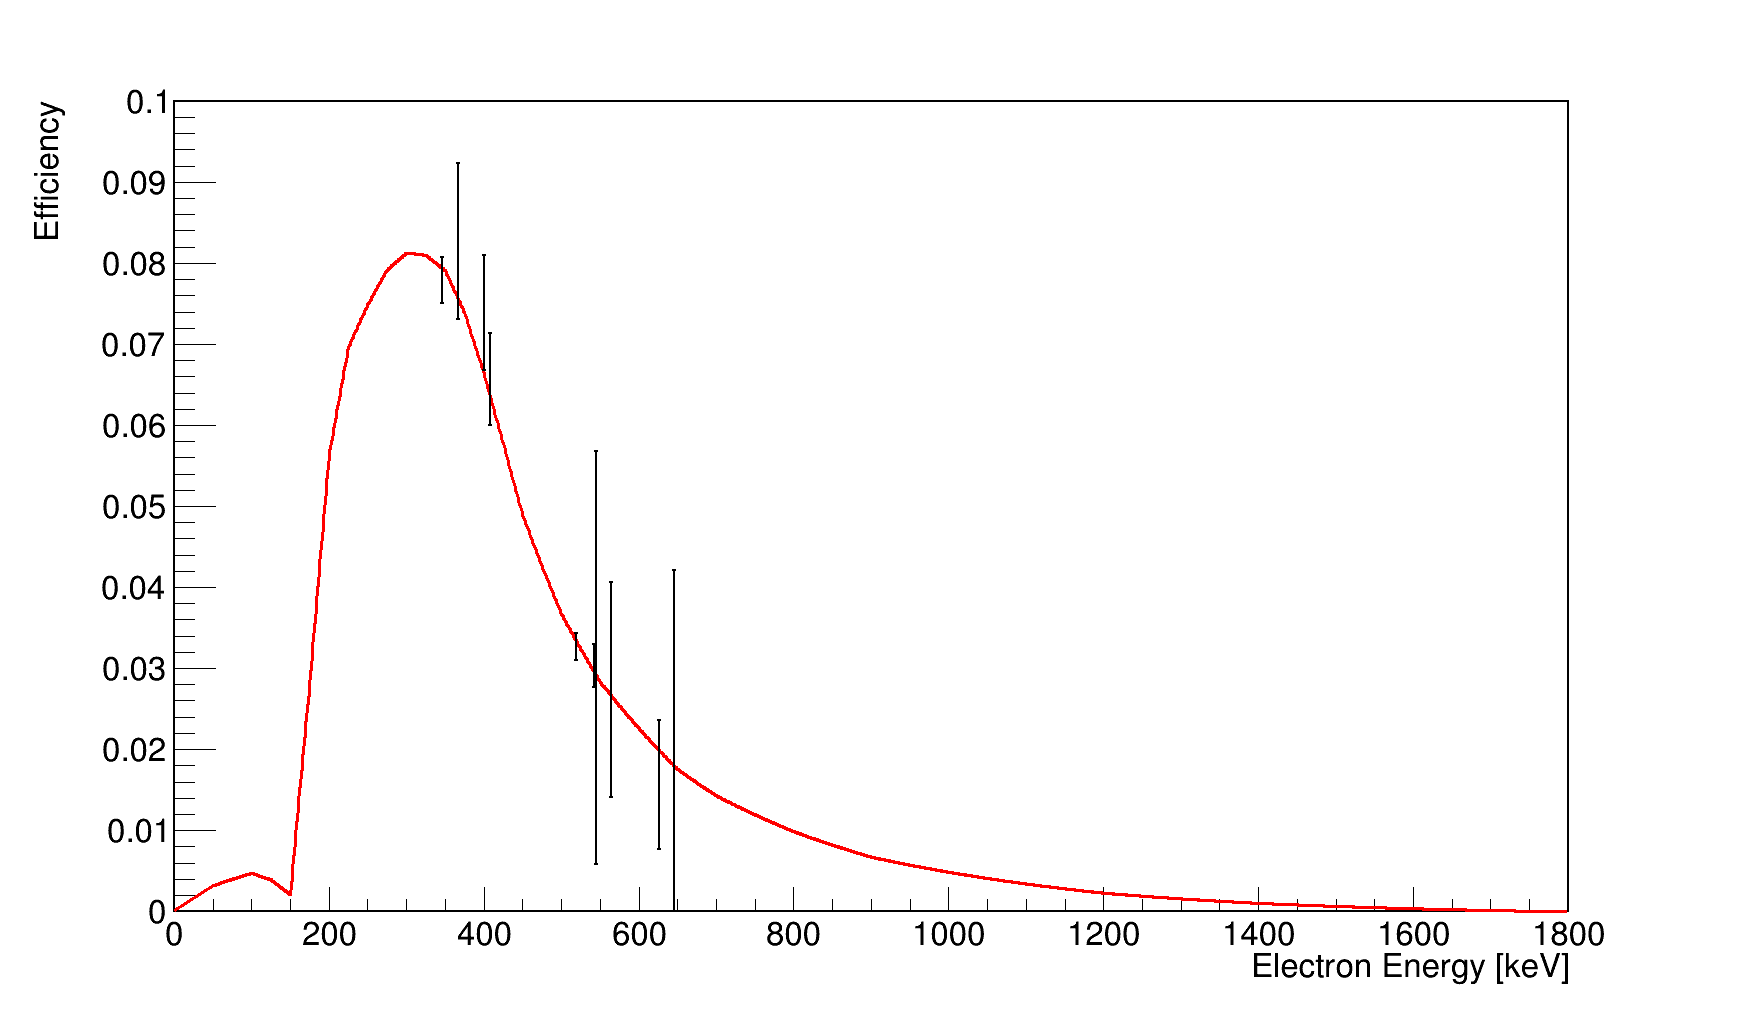
\includegraphics[width=\textwidth]{techniques_icc_scaled.png}
  \caption[The efficiency values and $K$ $e^-$ peak energies for several transitions are plotted and fit by an exponential scaling of the simulated SPICE efficiency curve.]{The efficiency values and $K$ $e^-$ peak energies for several transitions are plotted. The red curve represents the simulated SPICE efficiency curve, scaled by the fitted exponential function outlined in Equation (\ref{equation: exponential scaling}). The measurements used for this normalization routine are given in Table \ref{table:norm_icc}.}
  \label{figure: SPICE efficiency normalization with ICC measurements}
\end{figure}

% !!! When listing the spin assignments for states in this table, I've run into a question about dealing with tentative assignment. In the case of the highlighted transition from 109Pd, there is a lower energy state that is tentatively assigned as (7/2^+). Do I label the state here as the 'second' 7/2+ state with a '2' subscript? Sometimes only the parity or the spin are individually tentative. My approach has been to just leave off the numeric subscript whenever I encounter such ambiguity. 

\begin{sidewaystable}
  \begin{center}
    \begin{tabular}{|l|l l l|l l|l l|} 
     \hline
     & Transition & $E_\gamma \ [\mathrm{keV}]$ & Multipolarity & $\alpha_\mathrm{exp}(K) \times 10^3$ & $\alpha_\mathrm{exp}(L) \times 10^3$ &	$\epsilon_e (K)$ [\%]	& $\epsilon_e (L)$ [\%]\\  
     \hline
     $^{109}\mathrm{Pd}$	& $7/2^+ \rightarrow 5/2^+$	& 426.135	& $M1$	& 5.91(56)	& ---	& 7.39(71)	& --- \\
     						& $7/2^+ \rightarrow 5/2^+$	& 433.552	& $M1$	& 5.06(43)	& ---	& 6.57(57)	& --- \\
     $^{110}\mathrm{Pd}$	& $2_1^+ \rightarrow 0_1^+$ & 373.8  	& $E2$	& 10.27(33)	& 1.46(18)		& 7.78(28)	& 8.27(97)	  \\  
                         	& $4_1^+ \rightarrow 2_1^+$ & 547.04  	& $E2$	& 1.60(8)	& ---	& 3.27(17)	& ---  \\
                            & $0_2^+ \rightarrow 2_1^+$ & 572.89  	& $[E2]$& 1.4(11)	& ---	& 3.1(25)	& ---  \\
                            & $6_1^+ \rightarrow 4_1^+$ & 653.1  	& $[E2]$& 0.51(26)	& 0.04(12)		& 1.57(79)	& 1.1(31)	  \\  
     $^{111}\mathrm{Cd}$	& $15/2^- \rightarrow 11/2^-$ & 571.72 	& $E2$	& 1.48(13)	& 0.17(8)		& 3.03(27)	& 2.7(13)	  \\     
     \hline
    \end{tabular}
  \end{center}
  \caption[Table of normalization transitions used in determining $e^-$ detection efficiencies for internal conversion coefficient measurements.]{Table of normalization transitions used in determining $e^-$ detection efficiencies for internal conversion coefficient measurements. Square parentheses indicate a tentative multipolarity assignment.}
  \label{table:norm_icc}
\end{sidewaystable}

Since these are transitions of known multipolarity, the efficiency values for normalization are being calculated via the following relationship:

\begin{gather}
\epsilon_e= \frac{\alpha_\mathrm{exp}}{\alpha_\mathrm{BrIcc}} \cdot \epsilon_\gamma
\label{equation: Electron efficiency normalization}
\end{gather}

where $\alpha_\mathrm{BrIcc}$ is the theoretically calculated internal conversion coefficient from BrIcc \cite{KIBEDI2008202}.

%%%%%%%%%%%%%%%%%%%%%%%%%%%%%%%%%%%%%%%%%%%%%%%%
\section{Determining $E0$ Transition Strengths} \label{sec:Determining E0 Transition Strengths}
%%%%%%%%%%%%%%%%%%%%%%%%%%%%%%%%%%%%%%%%%%%%%%%%

Using the conversion coefficients determined in this experiment, along with previously measured experimental values such as the mixing ratio, $\delta(E2/M1)$, the $\rho^2(E0)$ value can be determined from \cite{Kibedi2005}

\begin{gather}
\rho^2(E0) = \frac{1}{\Omega_K(E0) \cdot \tau_K(E0)}
\label{equation: E0 strength via partial lifetimes}
\end{gather}

where $\Omega$ is the electronic factor obtained from BrIcc \cite{KIBEDI2008202} and $\tau(E0)$ is the partial mean lifetime of the $E0$ transition. The subscript $K$ denotes that the $E0$ strength is calculated for $K$ shell internal electron conversion. The partial mean lifetime, $\tau(E0)$, is calculated via

\begin{gather}
\tau(E0) = \frac{\Sigma \lambda_r}{\lambda_r(E0)} \cdot \tau
\label{equation: partial lifetime from relative decay constants}
\end{gather}

where $\tau = T_{1/2}/\ln(2)$ and $\lambda_r$ is the relative decay constant which is specific to each available decay mode from the parent state \cite{KraneText}. Hence the summation over all decay modes is performed in order to quantify the fractional value of the $E0$ lifetime relative to all other modes. An example is shown in Table \ref{table: inputs to the partial lifetime calculation of E0 strength} for the $2_2^+ \rightarrow 2_1^+$ transition in $^{110}\mathrm{Pd}$.

\begin{table}
  \begin{center}
    \begin{tabular}{|l|l|l|l|l|l|} 
     \hline
     $i$& Transition 					& Multipolarity & Mode 					& Method 					& $\lambda_r$ 			\\  
     \hline
     0	& A$(2_2^+ \rightarrow 2_1^+)$	& $E2$			& $\gamma$				& Set to 1					& 1						\\ 
     1	&								& 				& $e^-$					& $i_0 \cdot \alpha_K(E2)$	& $7.56 \times 10^{-3}$	\\ 
     2	&								& $M1$			& $\gamma$				& $i_0 / \delta^2$			& $4.72 \times 10^{-2}$	\\ 
     3	&								& 				& $e^-$					& $i_2 \cdot \alpha_K(M1)$	& $3.14 \times 10^{-4}$	\\ 
     4	&								& $E0$			& $e^-$					& $i_1 \cdot q_K^2$			& $-1.10 \times 10^{-4}$	\\ 
     5	& B$(2_2^+ \rightarrow 0_1^+)$	& 				& all					& 							& 0.37					\\
     \hline
     	&	A							&				& $\lambda_r(E0)$		& $i_4$ 					& $-1.10 \times 10^{-4}$	\\
    	&	A \& B						&				& $\Sigma \lambda_r$	&							& 1.42					\\
     \hline
    \end{tabular}
  \end{center}
  \caption[The calculation of $\lambda_r$ for each possible decay mode from the $2^+_2$ state in $^{110}$Pd.]{The calculation of $\lambda_r$ for each possible decay mode from the $2^+_2$ state in $^{110}$Pd. The errors are excluded in this table but are determined for the final value with a Monte Carlo method.}
  \label{table: inputs to the partial lifetime calculation of E0 strength}
\end{table}

The input $\delta(E2/M1)$ value carries a large, asymmetric uncertainty value. In a traditional approach to error propagation, a series of summations of real and fractional measurement error, in quadrature, would yield a final error estimate for $\rho^2(E0)$. However this approach is not applicable in instances of asymmetric error on inputs, and will yield an incorrect result. As such, the final value in this work is determined through a Monte Carlo method.

In the Monte Carlo method, each experimental value used as an input is assumed to be a normal distribution with a mean and width given by ($\mu, \sigma $). A simulation is performed, in which each event results in a calculation of $\rho^2(E0)$ using input values chosen at random from each distribution of ($\mu, \sigma$). These calculations, each instance being an iteration of Equation (\ref{equation: E0 strength via partial lifetimes}), fill a distribution of $\rho^2(E0)$ values. An example distribution for the $2_2^+ \rightarrow 2_1^+$ transition in $^{110}\mathrm{Pd}$ is shown in Figure \ref{figure: Monte Carlo distribution}.

\begin{figure}[!ht]
  \centering
  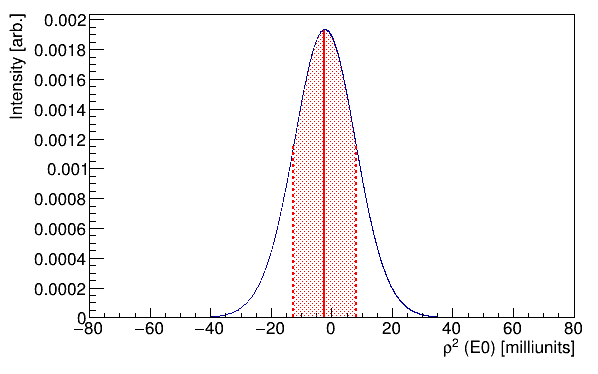
\includegraphics[width=\textwidth]{techniques_monte_carlo.png}
  \caption[An example distribution of $\rho^2(E0)$for the $2_2^+ \rightarrow 2_1^+$ transition in $^{110}\mathrm{Pd}$, produced by the Monte Carlo method.]{An example distribution of $\rho^2(E0)$for the $2_2^+ \rightarrow 2_1^+$ transition in $^{110}\mathrm{Pd}$, produced by the Monte Carlo method. The solid red line is the mean of the distribution and the shaded error is the $68\%$ confidence limit, or 1$\sigma$.}
  \label{figure: Monte Carlo distribution}
\end{figure}

In the example shown in Figure \ref{figure: Monte Carlo distribution} the mean of the distribution is in the unphysical ($< \ 0$) region. This result constitutes an effective measurement of zero, indicating a negligible $E0$ component to the transition. The negative, unphysical result is interpreted as a byproduct of measurement uncertainty and statistical methodology. An additional statistical finesse is required in order to interpret this result and extract a measurement. 

In a Bayesian statistical model, the approach of taking the product of this distribution with a `prior' distribution would be used. The prior distribution is a chosen function that represents all \textit{a priori} knowledge about the expected value. In this case, where $\rho^2(E0)$ is defined to be non-negative, a distribution that is constant for $x>0$, and zero for $ x \leq 0$ could be chosen. However this is considered to be an arbitrary solution \cite{GregoryText}. The alternative is the Neyman construction using the Feldman-Cousins ordering principle \cite{JamesText}. In this method, the distribution is used to determine the upper and lower limit in each true value of $\rho^2(E0)$, i.e. each y-slice in Figure \ref{figure: Monte Carlo distribution}. This construction assumes that the experimentally measured value of $\rho^2(E0)$ is representative of the unique experimental ensemble used to achieve the measurement. Implied is the existence of a distribution of experimental ensembles that could have been used to make the measurement, ensembles varying in their detector properties and other such systematics. The Neyman construction uses a frequentist statistical approach and yields confidence intervals describing the likelihood of the true $\rho^2(E0)$, as it exists in nature, coinciding with the measurement carried out by our experimental ensemble.

The Feldman-Cousins ordering principle is an alternative way of determining the confidence limits i.e. instead of simply rearranging the distribution from maximum to minimum, a separate ratio is calculated from \cite{JamesText}

\begin{gather}
R = \frac{P(x\rvert \mu)}{P(x\rvert \mu_\mathrm{best})}
\label{eq:feldman cousins}
\end{gather}

where $\mu_\mathrm{best}$ is the most likely value of $\mu$ in the physical (i.e. $x > 0$) region. The distribution is then ordered from the highest value of $R$ to the lowest and counted again until 68\% of the distribution is obtained. This method essentially adjusts coverage of the confidence region to remain in the physically allowed area. Using the distribution of Figure \ref{figure: Monte Carlo distribution}, the Feldman-Cousins ordering principle is used to determine the confidence limits for the Neyman construction in Figure \ref{figure: Neyman construction}. As the measured mean value is -2.325, a dashed line is drawn to determine the upper limit of +8.31. 

\begin{figure}[!ht]
  \centering
  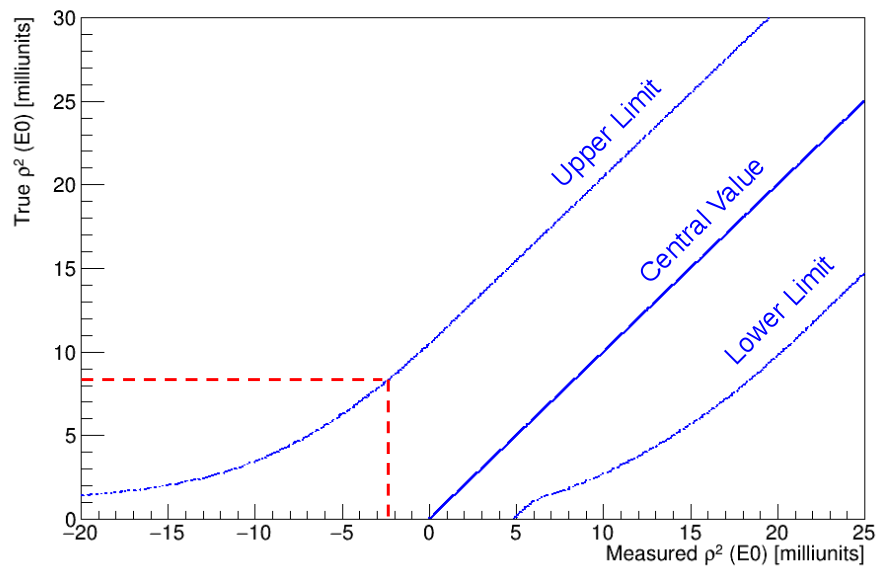
\includegraphics[width=\textwidth]{techniques_neyman.png}
  \caption[An example of the Neyman Construction produced using the distribution of Figure \ref{figure: Monte Carlo distribution}.]{An example of the Neyman Construction produced using the distribution of Figure \ref{figure: Monte Carlo distribution}. The measured mean value of the distribution was -2.325, a dashed line is drawn to determine the upper confidence limit of +8.31.}
  \label{figure: Neyman construction}
\end{figure}


\endinput

Any text after an \endinput is ignored.
You could put scraps here or things in progress.

%%%%%%%%%%%%%%%%%%%%%%%%%%%%%%%%%%%%%%%%%%%%%%
JTS from Paper
%%%%%%%%%%%%%%%%%%%%%%%%%%%%%%%%%%%%%%%%%%%%%%

{\it Experimental Details -}
% Beamtime was June 2016. TIGRESS elogs 14417 to 14687.
A beam of 35.6\,MeV alpha particles with a typical intensity of 120\,ppA was delivered by the TRIUMF-ISAC-II superconducting linear accelerator to the TIGRESS spectrometer. The beam was incident on a self-supporting $^{110}$Pd target of 1.6\,mg/cm$^2$ with a 97.61\% isotopic enrichment. The target was positioned 8\,mm upstream of the nominal center of the TIGRESS spectrometer.
Two micron S3 silicon detectors of 140\,$\mu$m and 1000\,$\mu$m thickness were located downstream in a $\Delta E-E$ telescope configuration to detect and identify charged particles. Twelve of the TIGRESS high-purity germanium (HPGe) clover detectors were positioned around the target location to detect $\gamma$ rays. Four clovers were located at 45$^{\circ}$ with respect to the beam axis, and the remaining eight at 90$^{\circ}$. Each clover was fully Compton suppressed and positioned at a target-to-detector distance of 14.5\,cm in the `Optimized peak-to-total' configuration of the TIGRESS spectrometer \cite{Hackman14}.

The spectrometer for internal conversion electrons (SPICE) detector was used to detect internal conversion electrons emitted from excited states populated in the reaction. The main detector of SPICE is a 6.1\,mm thick lithium-drifted silicon (Si(Li)) detector shielded by a photon shield from direct sight of the target. A magnetic lens formed of rare-earth permanent magnets collects and directs internal conversion electrons around the photon shield into the Si(Li) detector. The annular detector with inner and outer radii of 1 and 10\,cm is segmented into 120 individual segments arranged with 12 azimuthal sectors and 10 rings.

The detector signals were processed by the TIGRESS data acquisition system \cite{Martin08}. Data were collected when one of three hardware coincidence triggers between detector types was satisfied; [Si(Li) + S3], OR [Ge + S3] OR [Si(Li) + Ge]. In the case of S3 a pre-trigger coincidence between the delta-E and E detectors was required.

%%%%%%%%%%%%%%%%%%%%%%%%%%%%%%%%%%%%%%%%%%%%%%
Daniel's report
%%%%%%%%%%%%%%%%%%%%%%%%%%%%%%%%%%%%%%%%%%%%%%

The TRIUMF-ISAC Gamma-Ray Escape-Suppressed Spectrometer (TIGRESS) is a gamma- ray detector array situated at TRIUMF, Canada’s national laboratory for particle and nuclear physics. TIGRESS consists of up to 16 gamma-ray detectors; each detector contains 4 high- purity germanium (HPGe) crystals, which can provide high-resolution measurements of the detected gamma-ray energies. The HPGe detectors are highly segmented, which allows de- termination of the gamma-ray interaction location. Because of the high velocity of the beam, gamma-ray energy peaks are Doppler-shifted and broadened in an angle-dependent manner, and this position sensitivity allows the effect to be corrected.
When a gamma ray strikes the detector, there is a chance that it will scatter off the crystal and not deposit its full energy (known as Compton scattering). If a gamma ray scatters into an adjacent HPGe crystal, TIGRESS can add the partial energies of each hit and reconstruct the gamma-ray energy. The HPGe detectors are surrounded by scintillator shields made from bismuth germanate (BGO) and cesium iodide (CsI) crystals. These shields can detect gamma rays that escape the HPGe crystals without depositing their full energy, and then reject those gamma-rays from the collected HPGe spectrum. These techniques increase the peak-to-total ratio of the spectrum [4].
TIGRESS can be equipped with ancillary detectors, including SPICE, the Spec- trometer for Internal Conversion Electrons. When nuclei de-excite, there is a chance that
3
rather than emitting a gamma-ray, an electron is instead ejected from the atom. These electrons may be measured with SPICE, providing information about the multipolarity of different transitions. A primary aim is to measure transitions between two 0+ states, and determine electric monopole (E0) transition strengths [5]. SPICE may be equipped with an annular silicon detector positioned downstream of the target that can detect recoiling nuclei (called an "S3"), divided into 24 rings and 32 segments, allowing determination of both the angle θ and the angle φ of the recoiling particles. The recoil detector has the energy resolution to distinguish between recoils of different species, so more information about the kinematics of individual reactions can be obtained. Figure 1 shows the TIGRESS array and SPICE.